\begin{samplecase}
{\bf Astrophysical reaction rates : n + ${}^{187}$Os}\newline
With TALYS, astrophysical reaction rates can be calculated.
As sample case, we took the work done in
Ref.\cite{Segawa2007} where the ${}^{187}$Os(n,$\gamma$) was studied for
the derivation of the age of the galaxy withing the
Re-Os cosmochronology. 
\subsubsection{Case a: ${}^{187}$Os(n,$\gamma$) cross section}
First, the calculated ${}^{187}$Os(n,$\gamma$) was compared with experimental data,
using the following input file

\VerbatimInput{\samples n-Os187-astro-ng/org/talys.inp}

The results are given in Fig.\ref{os187ng}.
\subsubsection{Case b: ${}^{187}$Os(n,$\gamma$) astrophysical reaction rate}
Next, the astrophysical reaction rates for neutrons on ${}^{187}$Os are computed 
with the following input file

\VerbatimInput{\samples n-Os187-astro-rate/org/talys.inp}

which produces various output files in which the reaction rates as 
function of temperature are given.
The $(n,\gamma )$ rate as given in the file {\em astrorate.g} is   
{\small \begin{verbatim}
# header:
#   title: Os187(n,g) reaction rate
#   source: TALYS-2.0
#   user: Arjan Koning
#   date: 2023-12-14
#   format: YANDF-0.1
# target:
#   Z: 76
#   A: 187
#   nuclide: Os187
# reaction:
#   type: (n,g)
#   Q-value [MeV]:  7.989608E+00
#   E-threshold [MeV]:  0.000000E+00
# datablock:
#   quantity: reaction rate
#   columns: 4
#   entries: 30
##       T        reaction rate      MACS           G(T)
##   [10^9 K]      [cm3/mol/s]       [mb]            []
   1.000000E-04   1.255844E+09   5.124098E+05   1.000000E+00
   5.000000E-04   9.040671E+08   1.649672E+05   1.000000E+00
   9.999999E-04   7.231653E+08   9.330813E+04   1.000000E+00
   5.000000E-03   4.264272E+08   2.460604E+04   1.000000E+00
   1.000000E-02   3.303214E+08   1.347778E+04   1.000024E+00
   5.000000E-02   1.845430E+08   3.367398E+03   1.207792E+00
   9.999999E-02   1.470494E+08   1.897340E+03   1.645169E+00
   1.500000E-01   1.335211E+08   1.406650E+03   1.952226E+00
   2.000000E-01   1.263106E+08   1.152409E+03   2.198210E+00
.....................................
\end{verbatim} } \renewcommand{\baselinestretch}{1.07}\small\normalsize
\noindent
Similar same numbers can be found in the file for protons, etc.
In {\em astrorate.tot} the rates for all reactions can be found.

\end{samplecase}
\begin{figure}
\centering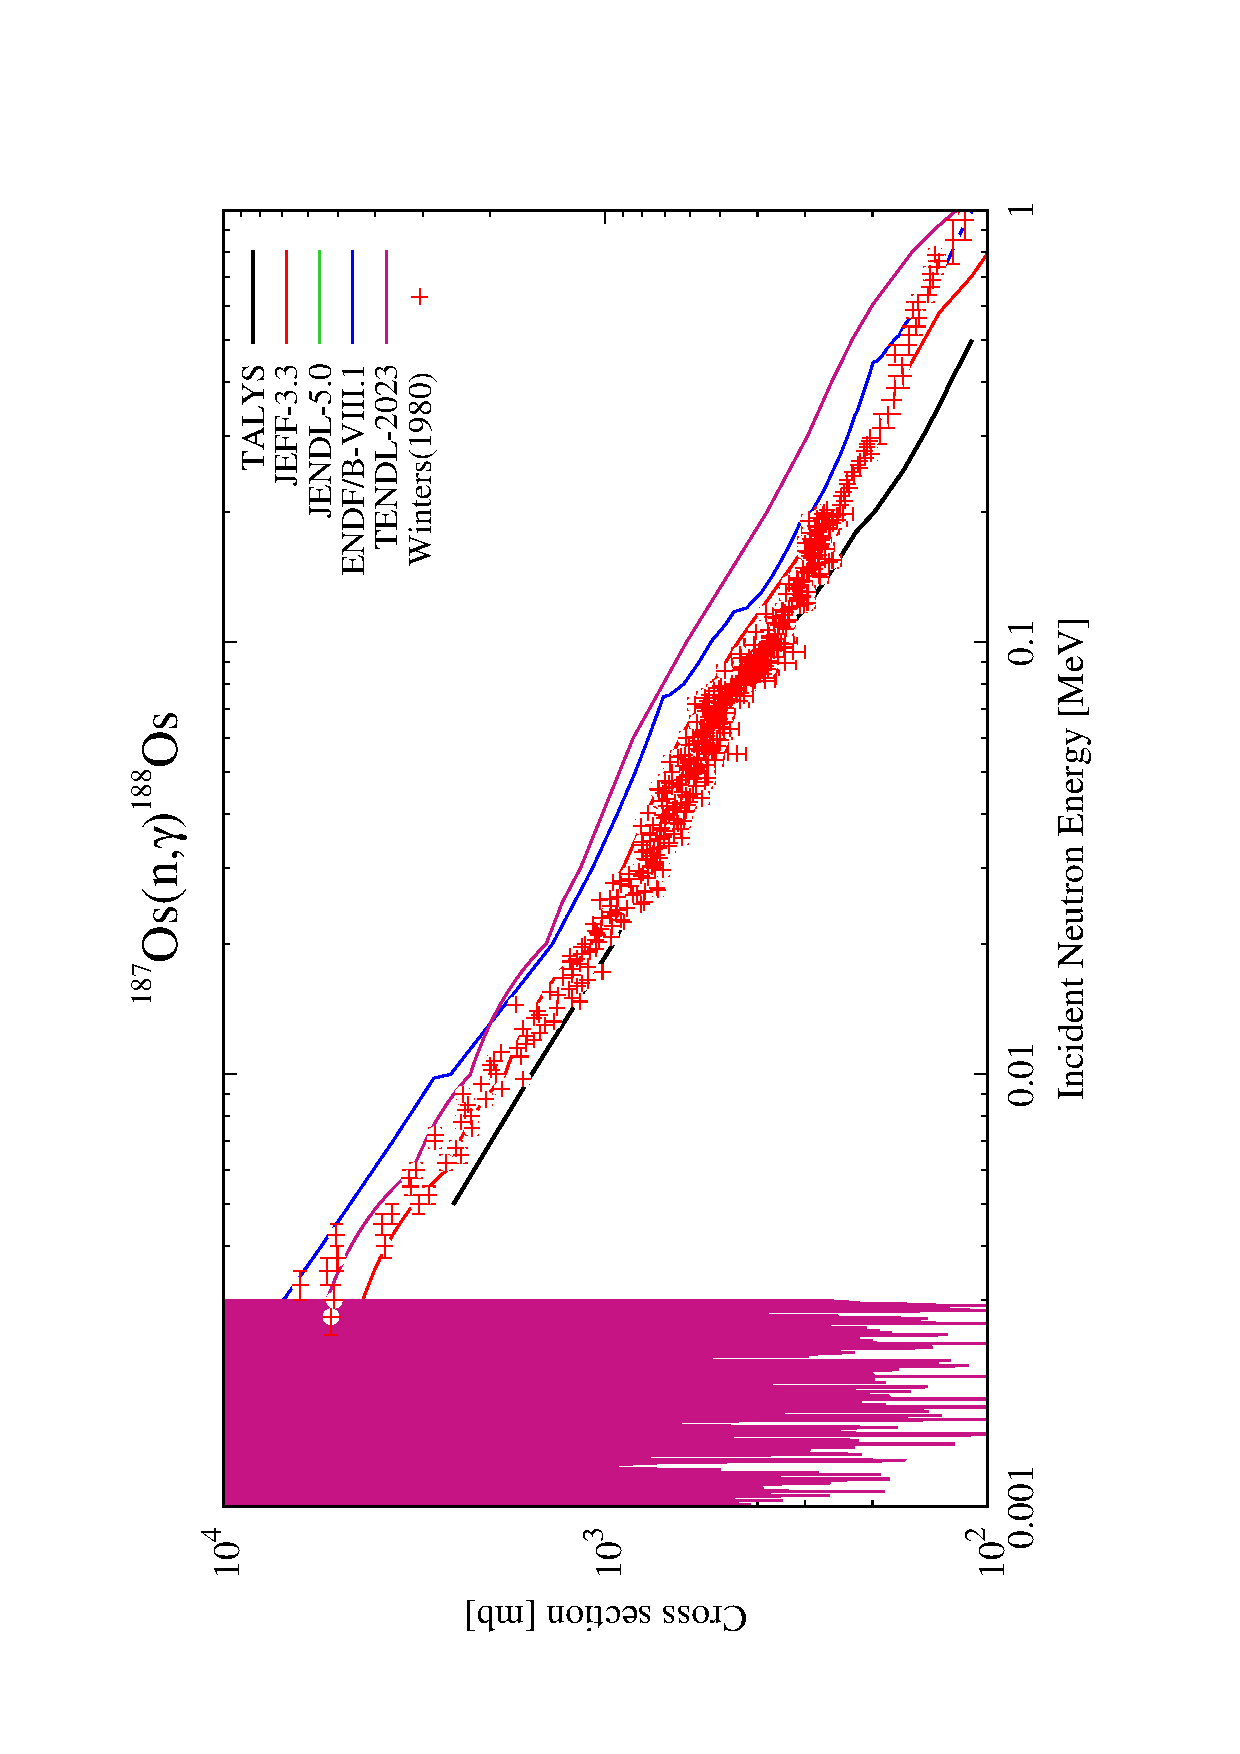
\includegraphics[scale=0.5,angle=270]{n-Os187-ng}
\caption{${}^{187}$Os(n,$\gamma$) cross section.}
\label{os187ng}
\end{figure}
